\documentclass[11pt]{beamer}
\usetheme{Pittsburgh}
\usepackage[utf8]{inputenc}
\usepackage{amsmath}
\usepackage{amsfonts}
\usepackage{amssymb}
\graphicspath{{../media/chpt1/}}
%\author{Author}
\title{MIMO Capacity Formula}
%\setbeamercovered{transparent} 
%\setbeamertemplate{navigation symbols}{} 
%\logo{} 
\institute{BITS Pilani} 
%\date{} 
\subject{first} 
\begin{document}

\begin{frame}
\maketitle
\end{frame}
\begin{frame}{Outline}
  \tableofcontents
\end{frame}

% Section and subsections will appear in the presentation overview
% and table of contents.
\section{Introduction to MIMO}


\begin{frame}{MIMO}
  \begin{itemize}
  \item Collection of signal processing techniques 
  \item Enhance performance (reliability/bandwidth) of wireless communication channels
  \item Using multiple antennas at Tx,Rx
  \item By exploiting multipath scattering properties of environment 
  \end{itemize}
\end{frame}
\begin{frame}{MIMO Techniques}
  \begin{enumerate}
    \item \textbf{spatial multiplexing :} Exploits multi-path fading to increase throughput without increasing the bandwidth requirement.
    Done by transmitting seperate data streams on each of the transmit antennas and seperating those streams by some form of spatial demultiplexing . eg. BLAST(Bell Labs Layered Space Time)
  \end{enumerate}
  \begin{figure}[H]
  \centering
  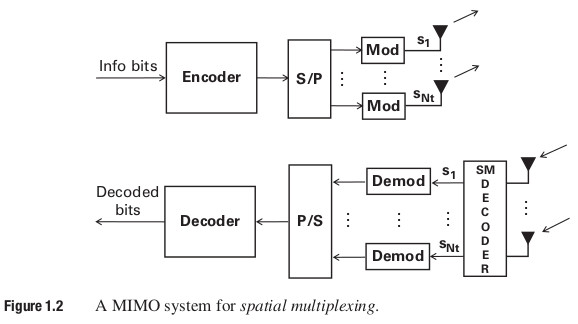
\includegraphics[scale=0.4]{spatial_multiplexing}
  \end{figure}
\end{frame}

\begin{frame}{MIMO Techniques}
  \begin{enumerate}
    \setcounter{enumi}{1}
    \item \textbf{spatial diversity :} Techniques that are used to improve reliability on a communications link by combating fading using 
    space-time coding . 
  \end{enumerate}
  \begin{figure}[H]
  \centering
  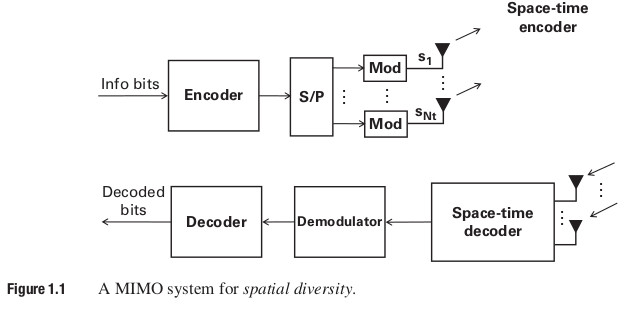
\includegraphics[scale=0.4]{spatial_diversity}
  \end{figure}
\end{frame} 


% Placing a * after \section means it will not show in the
% outline or table of contents.
\section*{Summary}

\begin{frame}{Summary}
  \begin{itemize}
  \item MIMO enchances performance of wireless communications channel
  \end{itemize}
\end{frame}



% All of the following is optional and typically not needed. 
\appendix
\section<presentation>*{\appendixname}
\subsection<presentation>*{For Further Reading}

\begin{frame}[allowframebreaks]
  \frametitle<presentation>{For Further Reading}
    
  \begin{thebibliography}{10}
    
  \beamertemplatebookbibitems
  % Start with overview books.

  \bibitem{Author1990}
    Jerry~R.~Hampton.
    \newblock {\em Introduction to MIMO Communications}.
    \newblock Cambridge University Press, 2014.
  \end{thebibliography}
\end{frame}


\end{document}